\chapter{Fundamentals}
\label{chapter:fundamentals}
\section{Machine learning: What and why?}
Machine learning is all about learning from data and gaining knowledge from it. Machine learning was initially thought of as automating
redundant human tasks and later developed into something that allowed solving complex
mathematical problems. It was seen just an addition to humans than extension of them.
Machine learning these days are required to perform tasks that are quite obvious and
natural to humans such as recognising faces in images or perceiving the road environment
around the vehicle and making decisions instinctively.

\begin{wrapfigure}{i}{0.5\textwidth}
	\centering
    \def\svgwidth{0.5\textwidth}
    \input{figures/inkscape/aimldl.pdf_tex} %use full path to know the location of pdftex
    \caption{Schema of AI, ML and DL}
    \label{fig:ai_ml_dl}
\end{wrapfigure}


All these attributes require to extend the field of machine learning.The figure \ref{fig:ai_ml_dl} shows how artificial
intelligence(AI) which was just a robot with simple if-else conditions, paved way for a
subset in Machine learning(ML) and ML in turn getting narrower focus to result in another
subset in Deep learning(DL).

So, in this chapter, a brief overview is given on the concepts that are implemented in the later chapters.

\subsection{Learning algorithms}
Machine learning provides a means to tackle tasks that are complex to solve through fixed
programmes and designed by human beings \cite{Goodfellow-et-al-2016}. A learning algorithm
is an algorithm which gains the ability to learn from data. A ML algorithm is one that
gains the ability to learn from an experience E with respect to some class of tasks T and
performance measure P \cite{mitchell1996m}. With experience, the algorithm can improve its
performance.

\subsubsection*{Tasks T}
The two major tasks in ML are \textit{classification} and \textit{regression}.

In classification related tasks, the system identifies which of \textit{k} categories an
input belongs to.

A function $f : \mathbb{R}^n \rightarrow\{1, \ldots,k\}$ is used by the
learning algorithm to solve this task. When $y = f(x)$, the model assigns an input
described by vector $\mathbf{x}$ to a category
identified by numeric code $y$. There are other variants of the classification
task, for example, where $f$ outputs a probability distribution over classes
\cite{Goodfellow-et-al-2016_1}. Alexnet \cite{Alexnet2012} is one of the examples of
classification task that used it to do object recognition.

Regression predicts continuous value output and at any given time for an appropriate
input to the neural network, regression will output a value corresponding to it.

A function $f: \mathbb{R}^n \rightarrow \mathbb{R}$ predicts a numerical value for some input.
Predicting the steering control value is a prime example for a regression task.

There are of course other tasks but only classification and regression are used in this
thesis. Hence the narrow focus.

\subsubsection*{Performance measure P}
To evaluate the performance of a ML algorithm, it is a must to design quantitative measure
of its performance. Usually this performance measure P is specific to a task T. There
are two distinct types of measurements -- accuracy and error rate.

If the goal is to learn a mapping from inputs $x$ to outputs $y$, where $y \in \{1,\ldots
, C\}$, with $C$ being the number of classes. If $C = 2$, this is
called binary classification (in which case we often assume $y \in \{0, 1\})$; if $C > 2$, this is called
multi class classification. If the class labels are not mutually exclusive (e.g., somebody may be
classified as tall and strong), we call it multi-label classification
\cite{murphy2013machine_1}.

Accuracy is just the proportion of examples for which the model produces the correct output.
So in the case of binary classification, if the function $f$ predicts a probability
densities $\hat y \in \{0.3, 0.7\}$, for a ground truth $y$ of value $1$, then P is $70\%$
accurate or the error rate is $30\%$.

It is essential that the model is evaluated with a data that it has not seen before. This data
\textit{testing set}, gives a good judgement on the performance  of the trained model.

\subsubsection*{Experience E}
The ML algorithms can be classified into \textit{supervised}, \textit{unsupervised} and
\textit{reinforcement} learning based on the kind of experience they are allowed to have.
A learning algorithm is allowed to gain experience by going through the \textit{dataset}.
A dataset is collection of all the examples for a given task. For example, to classify
which category a shown image belongs to has collection of images as dataset
\cite{cifar10}. Sometimes datasets are also called as \textit{data points}.

The focus will be on supervised learning in our case.  A random vector $\mathbf{x}$ explicitly attempts to
learn the probability distribution $p(\mathbf{x})$ and predicts $\mathbf{y}$ from
$\mathbf{x}$, usually estimating $p(\mathbf{y}\mid\mathbf{x})$. The CIFAR
dataset \cite{cifar10}, for example, contain images as features which inturn have \textit{targets} or
\textit{labels} associated with it. Here supervised learning(SL), the target
functionality(labels) is known. So it uses the images and predicts the probability
distribution to classify the images in the corresponding label.

\section{Deep Learning}
\label{chapter2sec:deeplearning}
Deep learning is a subset of machine learning. It takes all the algorithms, concepts from
 machine learning, and narrows the focus to enable a model to learn from data such that tasks
involve less human involvement, huge amount of data, and parameters.


\subsection{Simple neural network}
\textit{Linear regression} is one of the common SL algorithms. It solves the regression
problem. For example, if there is vector $\mathbf{x} \in \mathbb{R}^n$ as input and
predict a scalar value $y \in \mathbb{R}$ as its output, then in linear regression, output
is a linear function of the input. We can define it as
\begin{equation}
    \hat y = \mathbf{w}^T\mathbf{x}
    \label{eq:linear equation}
\end{equation}
where $\mathbf{w} \in \mathbb{R}^n$ is a vector of parameters.

\begin{wrapfigure}{l}{0.6\textwidth}
    \centering
        \def\svgwidth{0.55\textwidth}
        \documentclass[crop, tikz]{standalone}
\usepackage{tikz}

\usetikzlibrary{positioning}

\tikzstyle{inputNode}=[draw,circle,minimum size=10pt,inner sep=0pt]
\tikzstyle{stateTransition}=[-stealth, thick]

\begin{document}
\begin{tikzpicture}
	\node[draw,circle,minimum size=25pt,inner sep=0pt] (x) at (0,0) {$\Sigma$ $\sigma$};

	\node[inputNode] (x0) at (0, 1.75) {$\tiny +1$};
	\node[inputNode] (x1) at (-2, 0.75) {$\tiny x_1$};
	\node[inputNode] (x2) at (-2, 0) {$\tiny x_2$};
	\node[inputNode] (x3) at (-2, -0.75) {$\tiny x_3$};
	\node[inputNode] (xn) at (-2, -1.75) {$\tiny x_n$};

	\draw[stateTransition] (x0) to[out=-90,in=90] node [midway, right] {$b_0$} (x);
	\draw[stateTransition] (x1) to[out=0,in=150] node [midway, sloped, above] {$w_1$} (x);
	\draw[stateTransition] (x2) to[out=0,in=180] node [midway, sloped, above] {$w_2$} (x);
	\draw[stateTransition] (x3) to[out=0,in=210] node [midway, sloped, above] {$w_3$} (x);
	\draw[stateTransition] (xn) to[out=0,in=240] node [midway, sloped, above] {$w_n$} (x);
	\draw[stateTransition] (x) -- (4.2,0) node [midway,above] {$\sigma\left(w_0 + \sum\limits_{i=1}^{n}{w_ix_i}\right)$};
	\draw[dashed] (0,-0.43) -- (0,0.43);
	\node (dots) at (-2, -1.15) {$\vdots$};
	\node[inputNode, thick] (i1) at (6, 0.75) {$\tiny i_1$};
	\node[inputNode, thick] (i2) at (6, 0) {$\tiny i_2$};
	\node[inputNode, thick] (i3) at (6, -0.75) {$\tiny i_3$};
	
	\node[inputNode, thick] (h1) at (8, 1.5) {$\tiny h_1$};
	\node[inputNode, thick] (h2) at (8, 0.75) {$\tiny h_2$};
	\node[inputNode, thick] (h3) at (8, 0) {$\tiny h_3$};
	\node[inputNode, thick] (h4) at (8, -0.75) {$\tiny h_4$};
	\node[inputNode, thick] (h5) at (8, -1.5) {$\tiny h_5$};
	
	\node[inputNode, thick] (o1) at (10, 0.75) {$\tiny o_1$};
	\node[inputNode, thick] (o2) at (10, -0.75) {$\tiny o_2$};
	
	\draw[stateTransition] (5, 0.75) -- node[above] {$I_1$} (i1);
	\draw[stateTransition] (5, 0) -- node[above] {$I_2$} (i2);
	\draw[stateTransition] (5, -0.75) -- node[above] {$I_3$} (i3);
	
	\draw[stateTransition] (i1) -- (h1);
	\draw[stateTransition] (i1) -- (h2);
	\draw[stateTransition] (i1) -- (h3);
	\draw[stateTransition] (i1) -- (h4);
	\draw[stateTransition] (i1) -- (h5);
	\draw[stateTransition] (i2) -- (h1);
	\draw[stateTransition] (i2) -- (h2);
	\draw[stateTransition] (i2) -- (h3);
	\draw[stateTransition] (i2) -- (h4);
	\draw[stateTransition] (i2) -- (h5);
	\draw[stateTransition] (i3) -- (h1);
	\draw[stateTransition] (i3) -- (h2);
	\draw[stateTransition] (i3) -- (h3);
	\draw[stateTransition] (i3) -- (h4);
	\draw[stateTransition] (i3) -- (h5);
	
	\draw[stateTransition] (h1) -- (o1);
	\draw[stateTransition] (h1) -- (o2);
	\draw[stateTransition] (h2) -- (o1);
	\draw[stateTransition] (h2) -- (o2);
	\draw[stateTransition] (h3) -- (o1);
	\draw[stateTransition] (h3) -- (o2);
	\draw[stateTransition] (h4) -- (o1);
	\draw[stateTransition] (h4) -- (o2);
	\draw[stateTransition] (h5) -- (o1);
	\draw[stateTransition] (h5) -- (o2);
	
	\node[above=of i1, align=center] (l1) {Input \\ layer};
	\node[right=2.3em of l1, align=center] (l2) {Hidden \\ layer};
	\node[right=2.3em of l2, align=center] (l3) {Output \\ layer};
	
	\draw[stateTransition] (o1) -- node[above] {$O_1$} (11, 0.75);
	\draw[stateTransition] (o2) -- node[above] {$O_2$} (11, -0.75);
	
	\path[dashed, double, ultra thick, gray] (x.north) edge[bend left=0] (h5.north);
	\path[dashed, double, ultra thick, gray] (x.south) edge[bend right=0] (h5.south);
\end{tikzpicture}
\end{document}

        \caption{A simple neutral network}
        \label{fig:simpleNN}
\end{wrapfigure}


$\mathbf{w}$ is usually referred to as a set of weights that determine how each feature
affects the prediction. A $\mathbf{w}_i$ is simply multiplied with a feature $x_i$ to
predict $\hat y$. By manipulating the $\mathbf{w}_i$ value, the corresponding feature $x_i$ has
an effect on the prediction  $\hat y$.

A learning algorithm, in this case linear regression, is implemented as a perceptron. It
is a single-layer neural network as first suggested by Rosenblatt in 1958. They generally consist of four main parts -- input
nodes $x_i$, weights $w_i$, bias $b_0$(if necessary), net sum $\Sigma$ and an activation
function $\sigma$. This is shown in the figure \ref{fig:simpleNN}.

\subsection{Activation function}
\label{subsec:activationfunction}
The common activation functions used are Rectified Linear unit(ReLu), sigmoid, tanh and
softmax function. For each type of activation, $\sigma$ then decides if the input received is
relevant or not relevant. To convert linear inputs to non-linear, all that has to be done
is to use a non-linear activation function. The figure \ref{fig:activationfunctions},
shows the characteristics of some of the activation functions.

\begin{figure}[!ht]
	\begin{center}
   \def\svgwidth{0.8\textwidth}
    \input{figures/inkscape/activatefns1.pdf_tex} %use full path to know the location of pdftex
	\end{center}
    \caption{Activation functions}
    \label{fig:activationfunctions}
\end{figure}
For classification tasks, usually the last layer of the networks is equipped with softmax
activation layer. This function normalises the output to a probability distribution over
predicted output classes.

\begin{figure}[!ht]
    \def\svgwidth{0.8\textwidth}
	\begin{center}
        \input{figures/inkscape/inputhiddenoutput.pdf_tex} %use
    \end{center}
    \caption{Multi layer perceptrons}
    \label{fig:MLP}
\end{figure}

\subsection{Multilayer feedforward networks}
\label{subsec:MLP}
Deep feedforward networks or multilayer perceptrons are the quintessential deep learning
models. Its goal is to approximate function $f^*$. In the below figure \ref{fig:MLP},
information flows from inputs $\mathbf{x}$ to output $y$ using a mapping function
$\mathbf{y} = f(\mathbf{x};\mathbf{\theta})$ where $\theta$ are the parameters values
which the MLP learns for optimal approximation.

They are called feedforward as there are no feedback connections in which outputs of the
model are fed back into itself. Feedforward networks with feedbacks are called
\textit{recurrent neutral networks}.

Feedforward networks form the core for many commercial applications. For example, the
convolutional neural networks used for object detection are a special kind of feedforward
networks.

More the hidden layers, more the depth of the feedforward networks. Each hidden layer of the network is typically vector-valued.
The dimensionality of these hidden layers determines the width of the model. For eg. units
in MLP or feature maps in convolutional neural network.

\subsection{Loss function}
\label{subsec:lossfunction}
As mentioned before, a mapping function $f$ noisily approximates the input $x$ to output
$y$. So, the noise or the deviation from the true value(ground truth) must be kept at
minimum. The function that calculates the deviation is called \textit{cost} or
\textit{loss} function. It is important to choose the right loss function for a model.

\begin{figure}[!ht]
	\centering
    \def\svgwidth{0.6\textwidth}
    \input{figures/inkscape/mse.pdf_tex} %use full path to know the location of pdftex
    \caption{Mapping from x to y. The predictor is shown as linear line. The distance
    between the true values and predictor gives the loss. The sum of all the distances
gives the loss function.}
\label{fig:loss function}
\end{figure}

For multi-label classification tasks, \textit{categorical cross-entropy} function is used.
For each category, cross-entropy is calculated. The difference between the cross-entropy
of training data and the model's predictions is the cost function.
\begin{equation}
  CCE = -\frac{1}{N}\sum_{i = 1}^N [\hat{y_{i}}\log(y_{i})  + (1-
  \hat{y_{i}})\log(1-y_{i})]
   \label{eq:CCE}
\end{equation}

For regression tasks, the models are subjected to loss functions such as \textit{mean
absolute error}(MAE), \textit{mean squared error}(MSE) and \textit{mean squared
logarithmic error}(MSLE). In MAE, the mean of absolute differences among predictions and
expected results are calculated.
\begin{equation}
    MAE = \frac{1}{n}\sum_{i=1}^n\left |y_i -\hat y_i \right|
   \label{eq:MAE}
\end{equation}
In MSE, the mean of squared differences among predictions and true outputs are
calculated.
\begin{equation}
    MSE = \frac{1}{n}\sum_{i=1}^n (y_i - \hat y_i)^2
    \label{eq:MSE}
\end{equation}
In MSLE, the mean of relative distances between predictions and true outputs are
calculated.
\begin{equation}
    MSLE = \frac{1}{n}\sum_{i=1}^n(log(y_i+1)-log(\hat y_i+1))^2
    \label{eq:MSLE}
\end{equation}

\begin{wrapfigure}{I}{0.6\textwidth}
	\centering
    \def\svgwidth{0.6\textwidth}
        \input{figures/inkscape/minima.pdf_tex}
    \caption{Finding the global minima using gradient descent}
    \label{fig:gradientdescent}
\end{wrapfigure}


\subsection{Gradient descent}
\label{subsec:gradientdescent}
Gradient descent is an optimization algorithm to minimise the cost function parameterised by a
model parameter $\mathbf{w}$ in a function $f$. The first derivative(or gradient) gives the slope of the
cost function. Hence, to minimise it, direction opposite to the gradient is chosen.

The rate at the which the gradient step reduces is given by the \textit{learning rate}. It
is one of the important parameters in training a model. It is also easily controlled by
the user. Higher the learning rate, greater the step size of each gradient; possibly causing the
step to miss the global minima. Lower the learning rate, more the number of steps or training cycles
needed to reach the global minima. Greater care must be taken in choosing the learning
rate when training a model.

\subsection{Backpropagation}
\label{subsec:backpropagation}
Backpropagation is the practice of tuning the weights of a neural net based on the error rate (i.e. loss) obtained in the previous epoch (i.e. iteration).
Proper tuning of the weights ensures lower error rates, making the model reliable by increasing its generalization.
This practice is a part of model training these days.

At the heart of backpropagation is an expression for the partial derivative
$\frac{\partial C}{\partial \mathbf(w)}$ of the cost function C with respect to any weight w (or bias b) in the network. The expression tells us how quickly the cost changes when we change the weights and biases.
Since this method requires computation of the gradient of the error function at each
iteration step, we must guarantee the continuity and differentiability of the error
function. This can be achieved by using appropriate activation function such as tanh,
sigmoid etc.


\subsection{Optimizer}
\label{subsec:optimizer}
The loss function explains how far the predictions are compared to the true
outputs in a mathematical way. During training process, certain parameters can be tweaked
to help the loss function predict correct and optimised results. However, there are
question such as how to change them, by how much and when?

This is exactly optmizer's function. As explained in \ref{subsec:gradientdescent}, gradient
descent and learning rate form the core of optimizer's functionality. \textit{Stocastic
gradient descent}(SGD) is one of the oldest techniques in which gradients for all of
training examples are calculated on every pass. Hence, they are slow
and require much computation power. Some of the other popular optimizers are Adam
\cite{kingma2014adam}, Adagrad \cite{adagradpaper}, RMSprop \footnote{RMSprop is an unpublished, adaptive learning rate
method proposed by Geoff Hinton in Lecture 6e of his Coursera Class \cite{RMSProp}}. Adam stands for adaptive moment estimation.
It is a combination of all the advantages of two other extensions of SGD -- Adagrad and
RMSprop. Adam is computationally efficient, straight forward to implement, invariant to
diagonal rescale of the gradients, and less effort need to hyperparameters tuning.

\subsection{Challenges in Machine learning algorithms}
\begin{enumerate}
    \item Insufficient labelled data
    \item Poor quality data and irrelevant features
    \item Overfitting/underfitting a model
\end{enumerate}
\begin{figure}[!ht]
	\centering
    \def\svgwidth{0.7\textwidth}
   \input{figures/inkscape/overfitting.pdf_tex} %use full path to know the location of pdftex
    \caption{Relationship between capacity and error. Inspired from
    \cite{Goodfellow-et-al-2016}}
    \label{fig:overfittingunderfitting}
\end{figure}

The first two issues can be solved if the user is careful during data collection and does
preprocessing before feeding the data into the training model. However, if the training or
the test data is too small, the model is subject to underfitting or overfitting. Though
our aim is to reduce the error in the training set, we also need to reduce the error in
the test set. The gap between training and testing error is also an important parameter.

Underfitting occurs when the model is not able to obtain sufficiently low error value for
the training set. Overfitting happens when the neural network memorises the data from the
training data set and therefore performs poorly on the test data set. This, consequently,
does not let training and testing errors to converge. The sweet spot is to stop training the model when the testing error
increases while the training error  decreases \label{inside:formodelcheckpoint} Left of the optimal point, the model underfits. Right of
it, the model overfits. The figure \ref{fig:overfittingunderfitting} shows how the
relationship between capacity and error. Validation error is the error calculated for the test set.

\begin{figure}[!ht]
	\centering
    \def\svgwidth{0.6\textwidth}
   % \begin{Large}
    \documentclass[crop, tikz]{standalone}
\usepackage{tikz}
\usepackage{bm}
\usepackage{relsize}

\usetikzlibrary{positioning}

\begin{document}
\begin{tikzpicture}

	\node[circle, draw, thick] (i1) {};
	\node[circle, draw, thick, above=2em of i1] (i2) {};
	\node[circle, draw, thick, above=2em of i2] (i3) {};
	\node[circle, draw, thick, below=2em of i1] (i4) {};
	\node[circle, draw, thick, below=2em of i4] (i5) {};
	
	\node[circle, draw, thick, right=4em of i1] (h1) {};
	\node[circle, draw, thick, right=4em of i2] (h2) {};
	\node[circle, draw, thick, right=4em of i3] (h3) {};
	\node[circle, draw, thick, right=4em of i4] (h4) {};
	\node[circle, draw, thick, right=4em of i5] (h5) {};
	
	\node[circle, draw, thick, right=4em of h1] (hh1) {};
	\node[circle, draw, thick, right=4em of h2] (hh2) {};
	\node[circle, draw, thick, right=4em of h3] (hh3) {};
	\node[circle, draw, thick, right=4em of h4] (hh4) {};
	\node[circle, draw, thick, right=4em of h5] (hh5) {};
	
	\node[circle, draw, thick, right=4em of hh2] (o1) {};
	\node[circle, draw, thick, right=4em of hh4] (o2) {};
	
	\draw[-stealth, thick] (i1) -- (h1);
	\draw[-stealth, thick] (i1) -- (h2);
	\draw[-stealth, thick] (i1) -- (h3);
	\draw[-stealth, thick] (i1) -- (h4);
	\draw[-stealth, thick] (i1) -- (h5);
	\draw[-stealth, thick] (i2) -- (h1);
	\draw[-stealth, thick] (i2) -- (h2);
	\draw[-stealth, thick] (i2) -- (h3);
	\draw[-stealth, thick] (i2) -- (h4);
	\draw[-stealth, thick] (i2) -- (h5);
	\draw[-stealth, thick] (i3) -- (h1);
	\draw[-stealth, thick] (i3) -- (h2);
	\draw[-stealth, thick] (i3) -- (h3);
	\draw[-stealth, thick] (i3) -- (h4);
	\draw[-stealth, thick] (i3) -- (h5);
	\draw[-stealth, thick] (i4) -- (h1);
	\draw[-stealth, thick] (i4) -- (h2);
	\draw[-stealth, thick] (i4) -- (h3);
	\draw[-stealth, thick] (i4) -- (h4);
	\draw[-stealth, thick] (i4) -- (h5);
	\draw[-stealth, thick] (i5) -- (h1);
	\draw[-stealth, thick] (i5) -- (h2);
	\draw[-stealth, thick] (i5) -- (h3);
	\draw[-stealth, thick] (i5) -- (h4);
	\draw[-stealth, thick] (i5) -- (h5);
	
	\draw[-stealth, thick] (h1) -- (hh1);
	\draw[-stealth, thick] (h1) -- (hh2);
	\draw[-stealth, thick] (h1) -- (hh3);
	\draw[-stealth, thick] (h1) -- (hh4);
	\draw[-stealth, thick] (h1) -- (hh5);
	\draw[-stealth, thick] (h2) -- (hh1);
	\draw[-stealth, thick] (h2) -- (hh2);
	\draw[-stealth, thick] (h2) -- (hh3);
	\draw[-stealth, thick] (h2) -- (hh4);
	\draw[-stealth, thick] (h2) -- (hh5);
	\draw[-stealth, thick] (h3) -- (hh1);
	\draw[-stealth, thick] (h3) -- (hh2);
	\draw[-stealth, thick] (h3) -- (hh3);
	\draw[-stealth, thick] (h3) -- (hh4);
	\draw[-stealth, thick] (h3) -- (hh5);
	\draw[-stealth, thick] (h4) -- (hh1);
	\draw[-stealth, thick] (h4) -- (hh2);
	\draw[-stealth, thick] (h4) -- (hh3);
	\draw[-stealth, thick] (h4) -- (hh4);
	\draw[-stealth, thick] (h4) -- (hh5);
	\draw[-stealth, thick] (h5) -- (hh1);
	\draw[-stealth, thick] (h5) -- (hh2);
	\draw[-stealth, thick] (h5) -- (hh3);
	\draw[-stealth, thick] (h5) -- (hh4);
	\draw[-stealth, thick] (h5) -- (hh5);
	
	
	\draw[-stealth, thick] (hh1) -- (o1);
	\draw[-stealth, thick] (hh1) -- (o2);
	\draw[-stealth, thick] (hh2) -- (o1);
	\draw[-stealth, thick] (hh2) -- (o2);
	\draw[-stealth, thick] (hh3) -- (o1);
	\draw[-stealth, thick] (hh3) -- (o2);
	\draw[-stealth, thick] (hh4) -- (o1);
	\draw[-stealth, thick] (hh4) -- (o2);
	\draw[-stealth, thick] (hh5) -- (o1);
	\draw[-stealth, thick] (hh5) -- (o2);
	
	\draw[-stealth, double, dashed, thick] (5.5,0) -- node[above] {dropout} (8.6, 0);
	
	
	%%% BOUNDARY %%%
	
	\node[circle, draw, thick, red, fill=red!10, right=15em of hh1] (i1) {};
	\node[circle, draw, thick, red, fill=red!10, above=2em of i1] (i2) {};
	\node[circle, draw, thick, above=2em of i2] (i3) {};
	\node[circle, draw, thick, below=2em of i1] (i4) {};
	\node[circle, draw, thick, below=2em of i4] (i5) {};
	
	\node[red] (icr) at (i1) {$\mathlarger{\mathlarger{\mathlarger{\mathlarger{\mathlarger{\bm{\times}}}}}}$};
	\node[red] (icr) at (i2) {$\mathlarger{\mathlarger{\mathlarger{\mathlarger{\mathlarger{\bm{\times}}}}}}$};
	
	\node[circle, draw, thick, red, fill=red!10, right=4em of i1] (h1) {};
	\node[circle, draw, thick, right=4em of i2] (h2) {};
	\node[circle, draw, thick, red, fill=red!10, right=4em of i3] (h3) {};
	\node[circle, draw, thick, red, fill=red!10, right=4em of i4] (h4) {};
	\node[circle, draw, thick, right=4em of i5] (h5) {};
	
	\node[red] (icr) at (h1) {$\mathlarger{\mathlarger{\mathlarger{\mathlarger{\mathlarger{\bm{\times}}}}}}$};
	\node[red] (icr) at (h3) {$\mathlarger{\mathlarger{\mathlarger{\mathlarger{\mathlarger{\bm{\times}}}}}}$};
	\node[red] (icr) at (h4) {$\mathlarger{\mathlarger{\mathlarger{\mathlarger{\mathlarger{\bm{\times}}}}}}$};
	
	\node[circle, draw, thick, right=4em of h1] (hh1) {};
	\node[circle, draw, thick, red, fill=red!10, right=4em of h2] (hh2) {};
	\node[circle, draw, thick, right=4em of h3] (hh3) {};
	\node[circle, draw, thick, red, fill=red!10, right=4em of h4] (hh4) {};
	\node[circle, draw, thick, right=4em of h5] (hh5) {};
	
	\node[red] (icr) at (hh2) {$\mathlarger{\mathlarger{\mathlarger{\mathlarger{\mathlarger{\bm{\times}}}}}}$};
	\node[red] (icr) at (hh4) {$\mathlarger{\mathlarger{\mathlarger{\mathlarger{\mathlarger{\bm{\times}}}}}}$};
	
	\node[circle, draw, thick, right=4em of hh2] (o1) {};
	\node[circle, draw, thick, right=4em of hh4] (o2) {};
	
	\draw[-stealth, thick] (i3) -- (h2);
	\draw[-stealth, thick] (i3) -- (h5);
	\draw[-stealth, thick] (i4) -- (h2);
	\draw[-stealth, thick] (i4) -- (h5);
	\draw[-stealth, thick] (i5) -- (h2);
	\draw[-stealth, thick] (i5) -- (h5);
	
	\draw[-stealth, thick] (h2) -- (hh1);
	\draw[-stealth, thick] (h2) -- (hh3);
	\draw[-stealth, thick] (h2) -- (hh5);
	\draw[-stealth, thick] (h5) -- (hh1);
	\draw[-stealth, thick] (h5) -- (hh3);
	\draw[-stealth, thick] (h5) -- (hh5);
	
	\draw[-stealth, thick] (hh1) -- (o1);
	\draw[-stealth, thick] (hh1) -- (o2);
	\draw[-stealth, thick] (hh3) -- (o1);
	\draw[-stealth, thick] (hh3) -- (o2);
	\draw[-stealth, thick] (hh5) -- (o1);
	\draw[-stealth, thick] (hh5) -- (o2);

\end{tikzpicture}
\end{document}

    %\end{Large}
    \caption{Illustrating dropout functionality}
    \label{fig:Dropout_function}
\end{figure}

\subsection{Regularization techniques}
DNNs contain multiple non-linear hidden layers which make them learn
complex relationships between their inputs and outputs. With a small training set, this
relationship adds sampling noise that won't exist in the real-world data even if drawn
from the same distribution. This leads to overfitting and several methods have been
developed to reduce its effect.
\begin{enumerate}
    \item Early stopping as soon as the validation error gets worse than the training
        error. \label{item:earlystopping}
    \item L1 and L2 regularisation which penalises the weights \cite{Schmidhuber_2015}.
    \item Randomly drop units(along with their connection) from the neutral network during
        training \cite{dropoutpaper}. Figure \ref{fig:Dropout_function} illustrates how to
        do the random dropping of units.
\end{enumerate}
\begin{figure}[!ht]
    \centering
    \def\svgwidth{\textwidth}
    \input{figures/inkscape/earlyfusion3.pdf_tex}
    \caption{CNN architecture}
    \label{fig:cnnarchitecture}
\end{figure}

\subsection{Convolution Neutral Network - CNN}
Convolutional neural network(CNN) or in short convnets is a deep learning algorithm for object recognition
tasks. What makes CNN stand out for image analysis? The network takes images as inputs, reduces them into a form
easier to process, without losing features which are critical for a good prediction. So
not only this is important to consider while designing an architecture but also while
scaling massive dataset.
\subsubsection*{Convolution Layer}
\label{subsubsec:convlayer}
The images which are taken as inputs are just n-dimensional matrix with pixel values. So a
convolution operation can be easily carried on it using a filter or \textit{kernel}. A
kernel matrix is pre-defined according to the task. Usually the size of the kernel is tiny
compared to that of the images which facilitates easy
convolution. A \textit{stride} is the value of a step taken by the kernel after each
convolution. If stride = 1, then it is called \textit{non-strided}. Convolution remarkably
extracts the high-level features such as edges. Normally there are many convnets in an
architecture. Each layer extracts a different feature or expands on last layer's task.

If the dimensionality of the convolved feature stays the same or increased compared to the
input, then it is called \textit{same padding}. If the dimensionality is reduced, its
\textit{valid padding}. Padding is extremely useful for solving boundary conditions.

\subsubsection*{Pooling Layer}
\label{subsubsec:pooling}
This layer is similar to convolutional layer. Its task is to decrease the computational
power required to process data, usually done through reducing the dimensionality. It is,
furthermore, useful to extract dominant features that are rotational and positional
invariant, thus maintaining the goal of training the model.

There are two types of pooling -- \textit{max pooling} and \textit{average pooling}. Max Pooling
returns the maximum value from the portion of the image covered by the kernel.
On the other hand, average Pooling returns the average of all the values
from the portion of the image covered by the kernel. Pooling also helps in reducing the
noisy pixels which sometimes skew feature extraction.

\subsubsection*{Flatten and Fully Connected Layer}
The main goal for extracting features from the images is to do some task; for example -
classification. So the extracted features must be converted into a form understandable for
the MLP (\ref{subsec:MLP}), which happens to be 1-dimensional vector. This is exactly the
task of \textit{flatten layer}.

MLP gets a vector as input and feeds it to a feedforward network in \textit{fully
connected layer}. Fully connected layer then outputs the necessary values depending on the
task.

It is important to remember that each layer employs an activation function(
\ref{subsec:activationfunction}) to introduce linearity or non-linearity to the inputs.

\subsection{Recurrent neural networks - RNN}
One of the drawbacks of neural networks is that they always start from scratch; with no
memory of the previous state. If a neural network has to be used for word prediction,
knowledge of previous letter and word is necessary. Recurrent neural networks addresses
this issue.

RNN provide the temporal dynamic behaviour. A typical RNN looks like in the figure
\ref{fig:RNN}. The left hand side shows it folded and right hand side unfolded in time.
\begin{figure}[!ht]
	\centering
        \def\svgwidth{1.0\textwidth}
        \input{figures/inkscape/simplernn.pdf_tex}
    \caption{A Simple RNN}
    \label{fig:RNN}
\end{figure}
RNN, however, suffers from \textit{long term dependencies}. This is well explored in
\cite{RNNdrawback1} and \cite{RNNdrawback2}.

\subsection{LSTM}
\label{subsubsec:lstm}
The shortcomings of RNN are overcome by LSTM - \textit{Long Short Term Memory}.
They are a special kind of RNN which was first introduced by Hochreiter \textit{et al.} \cite{LSTMPaper}. They remember
information for long periods as their default behaviour with ease. The figure
\ref{fig:lstm} shows how the structure of a LSTM differs from simple RNN. The LSTM employs
gates and activation functions to add or delete information from the previous state.

\begin{figure}[!ht]
    \centering
	   \def\svgwidth{0.7\textwidth}
    \input{figures/inkscape/lstm1.pdf_tex} %use full path to know the location of pdftex
    \caption{LSTM Architecture - Rolled}
    \label{fig:lstm}
\end{figure}

\begin{figure}[!ht]
    \centering
        \def\svgwidth{1.0\textwidth}
        \input{figures/inkscape/unrolledLSTM.pdf_tex} %use full path to know the location of pdftex
    \caption{LSTM Architecture - Unrolled}
    \label{fig:lstmunrolled}
\end{figure}
\newpage
\section{Sensors}
Deep neural networks need data -- images or measurements to perform necessary tasks. These
information/data are captured using sensors.
\subsection{Visual Sensors}
Visual sensors are one of the commonly used sensors for image capture of the environment.
Usually cameras are used.
\begin{figure}[!ht]
	\centering
    \def\svgwidth{0.6\textwidth}
        \input{figures/inkscape/rgbcamerasensor2.pdf_tex} %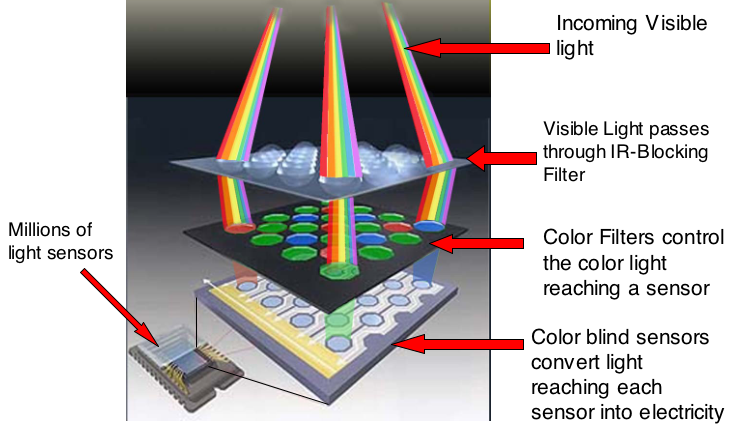
\includegraphics[width=0.6\textwidth]{figures/inkscape/rgbcamerasensor1.png}
    \caption{Inside RGB camera}
    \label{fig:rgbcamera}
\end{figure}

\subsubsection*{RGB Colour Camera}
A camera uses the lens to focus and captures objects. The information travels in the form of electro-magnetic waves such as light. The sensor
that is present behind the lens are made of photodetectors, is exposed to allow incoming
light. An variable electric charge is produced depending on the intensity of the light
waves. The intensity of the light waves changes with object's exposure. These charges are then quantified and stored as numerical values called
\textit{pixels}.

A pixel is generally the smallest single component of an image. Each pixel are arranged
one after another in the form of matrices. So, for a resolution of "640 x 480" display,
they are 640 pixels side to side and 480 from top to bottom.
A colour image is captured by using a colour filter such as Bayer filter to filter out
only light waves that are of RGB colour spectrum wavelength. Each pixel are then coded
in \textit{bits}. In our case we use eight bits to represent an image.


\subsubsection*{Depth Camera}
A depth camera is usually a stereo camera with two cameras. They are displaced
horizontally from one another. They are used to obtain two differing views on a scene.
Images are captured from these points and comparing the pixel values gives the relative position of
the objects.
\begin{figure}[!ht]
	\centering
    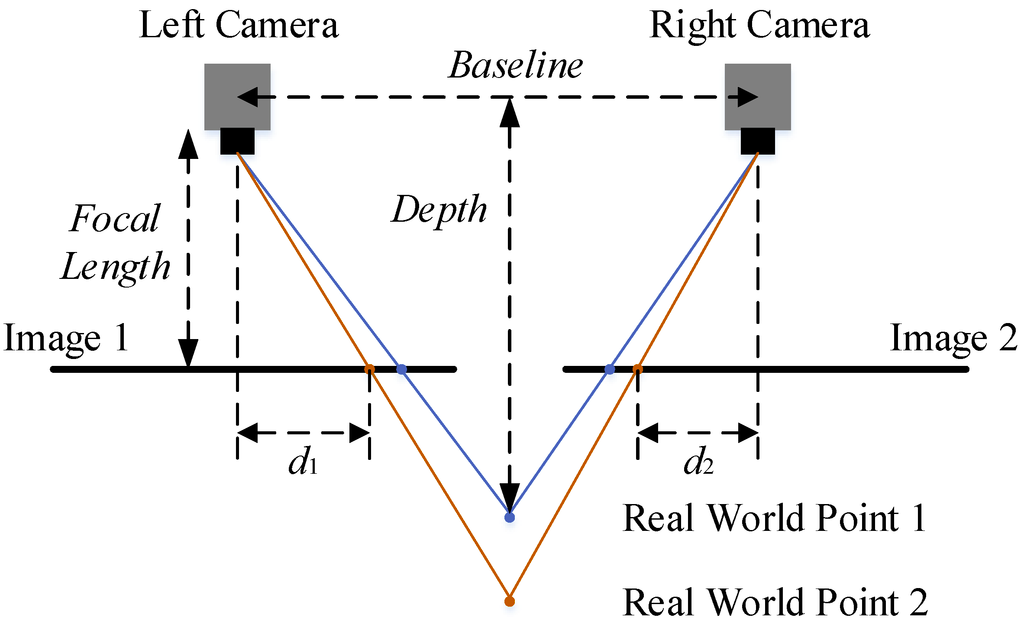
\includegraphics[width=0.6\textwidth,
    scale=0.1]{figures/inkscape/depthsensor2.png}
    \caption{How depth sensor works. Figure redrawn using a website
    \cite{depthstereodiagramsource} as reference.}
    \label{fig:depthcamera}
\end{figure}
A Depth camera sensor, captures images just like
a colour camera but only as grayscale images -- black and white pixels. These pixels are
then stored with eight bits per pixel(shades of grey). The shades on the grey-scale correspond to the depth of objects.
This paper \cite{depthsensorpaper1} shows how to combine  a  low  resolution
Time-Of-Flight  (TOF)  depth  image  camera based on Photonic Mixer Devices with two
standard cameras in a stereo configuration and without accurate calibration. And this
paper \cite{depthsensorpaper2} gives the basics on stereo camera for object perception.
\subsubsection*{Segmentation Camera}
RGB images are fed to CNN-DNN which groups the pixels of similar attributes using a
process called image segmentation. The most common image segmentation method is
thresholding. Pixels with certain threshold are grouped together. This allows to images to
have segments that may be more meaningful to analyse those segments than the whole image
for relevant information.

For autonomous driving, semantic segmentation method is used. RGB images are fed to a DNN
to group pixels according to user-defined tag. For example, a car is blue, pedestrian red, road boundaries white etc.
This paper by Poudel \textit{et al} \cite{segmentationpaper} uses encoder-decoder
architecture to do offline semantic image segmentation.

\subsection{Measurement Sensors}
These sensors are required for providing information other than visual such as telemetry
data.
\begin{figure}[!ht]
	\centering
    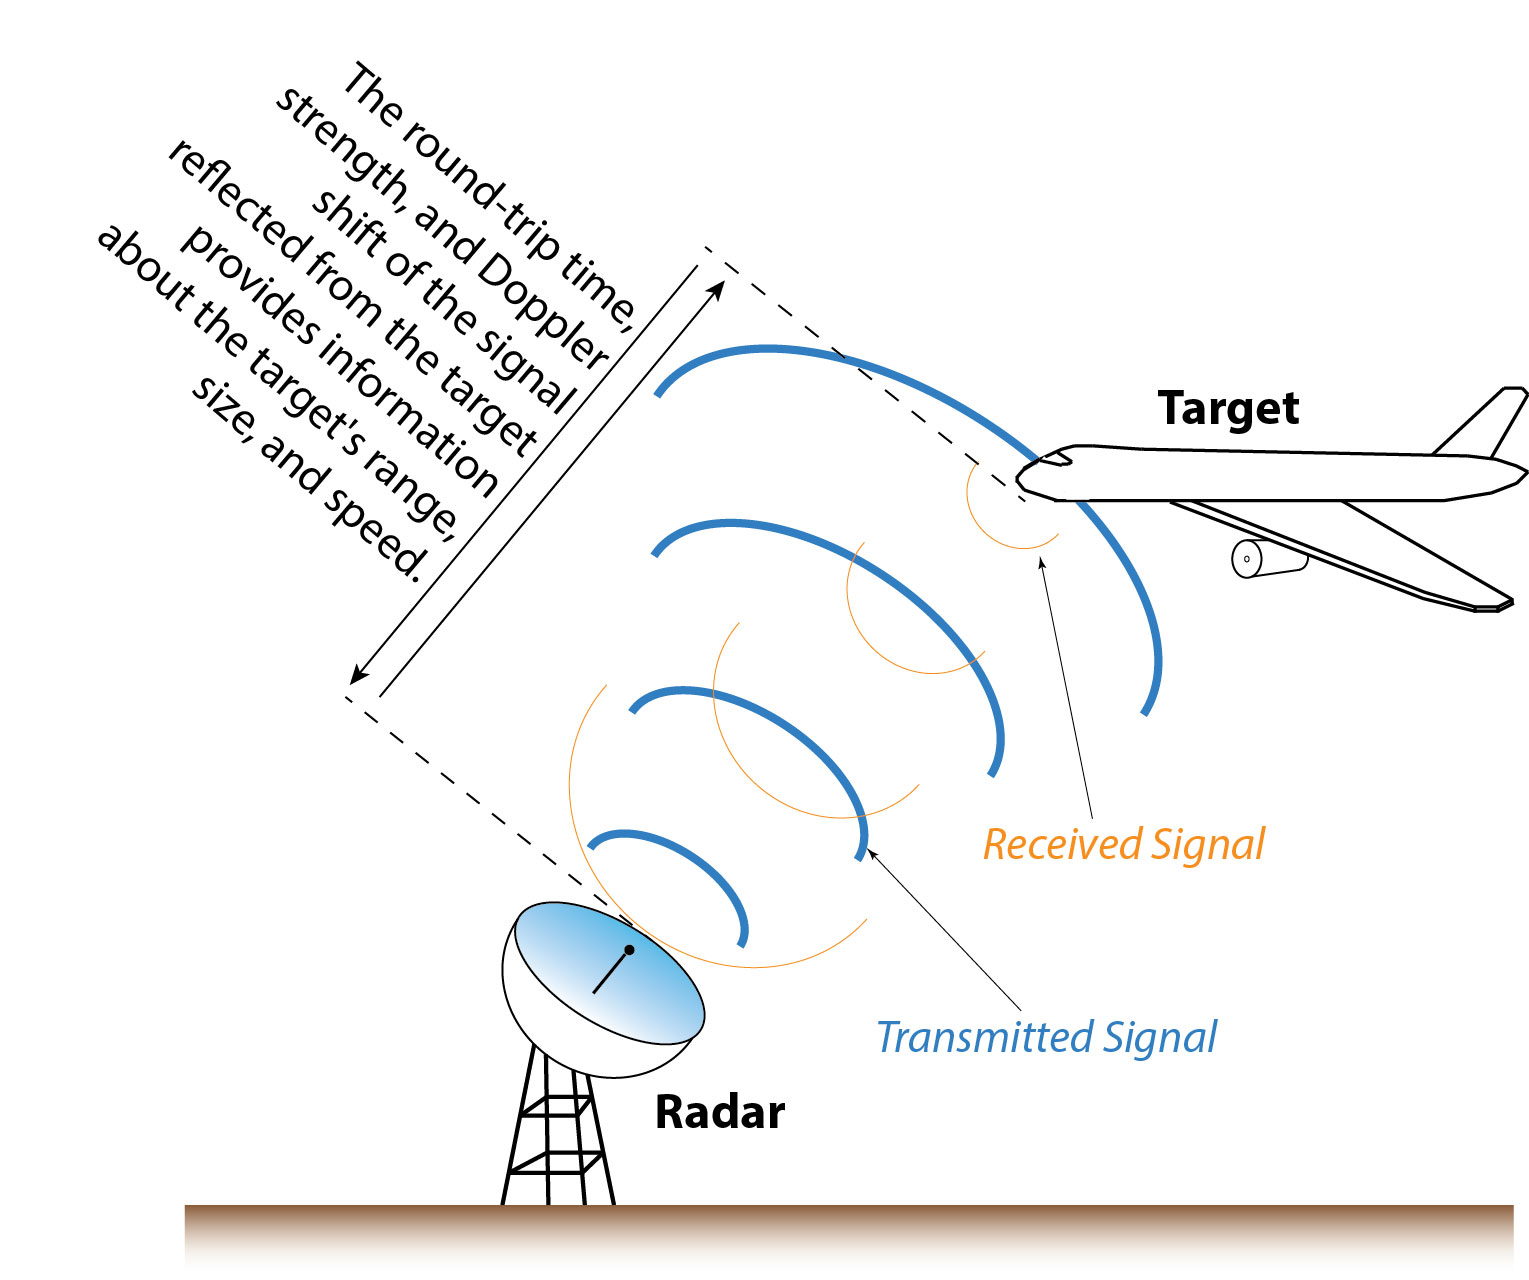
\includegraphics[width=0.6\textwidth, scale=0.1]{figures/inkscape/RadarFig.jpg}
    \caption{How radar works}
    \label{fig:radarsensor}
\end{figure}

\subsubsection*{Radar Sensor}
Radar is a detection system that uses electro-magnetic waves(radio waves) to determine the
range and velocity of objects. A common sensor that is used in weather forecast which is known for its
long range sensing and resistance to adverse weather conditions. It consists of a transmitting antenna with a
transmitter producing radio or microwave waves, a receiving antenna and receiver to
process the information. Radio waves reflect off the object and return to the receiver
carrying the information about object's velocity and position.
If the object is moving either toward or away from the transmitter, there will be a slight change in the frequency of the radio waves due to the Doppler effect.

Three major classes of radar systems are typically employed in automotive active safety systems:
\begin{enumerate}
    \item Short-range radar (SRR) for collision proximity warning and safety, and to support limited parking assist features.
    \item Medium-range radar (MRR) (24GHz) to watch the corners of the vehicle, perform blind spot detection, observe other-vehicle lane crossover and avoid side/corner collisions.
    \item Long-range radar (LRR) (77GHz) for forward-looking sensors, adaptive cruise control (ACC) and early collision detection functions.
\end{enumerate}

However, in LGSVL simulator, only high-level implementation of radar is implemented. It
does not use any waves, reflection or occlusion techniques. Since the simulator is aware
of vehicles' position at any given moment in the map, the information is converted to
depth information and stored.

\subsubsection*{Control Sensor}
With this sensor, telemetry information can be collected. This is usually done by
encoding the key presses in the keyboard.

\section{Sensor/Data Fusion}
\label{sec:datafusion}
To allow DNNs to make the best perception of the environment, it is necessary to fuse data from
several sensors and feed that combined data into the DNN. This technique of fusing
information exists for decades \cite{Datafusion1}. Often used data fusion technique is
\textit{Kalman filtering} and its variant \cite{Datafusion3} \cite{Datafusion2}. \cite{kalmanfilterpaper1},
\cite{kalmanfilterpaper2} give a comparison in performance between using Kalman filter and
LSTMs. \cite{kalmanfilterpaper3} uses recurrent YOLO(LSTMs) to track objects through space and time.

For autonomous driving, RGB and depth information(RGB-D) is vital for obstacle avoidance.
\cite{XiaoCodevillaMultimodalE2E} uses data fusion to get better results for their
experiment.
\subsection{Types of Data Fusion}
There are two traditional approaches to data fusion -- \textit{early fusion} and
\textit{late fusion}.
In early fusion, all the sensor inputs are concatenated before being fed to the CNN.
Whereas in late fusion, each sensor inputs are fed to separate convolutional layer and
down the line, they are concatenated together.

These techniques can be seen in action in this \cite{wang2020makes} recently
published paper from Facebook research team.
\begin{figure}[!ht]
	\begin{center}
        \def\svgwidth{\textwidth}
        \input{figures/inkscape/datafusionfrompaper2.pdf_tex}
	\end{center}
    \caption{This figure is taken from this \cite{Datafusion4} paper where they describe early and
        late fusion architectures and also present three types of late fusion.}
    \label{fig:Datafusiontypes}
\end{figure}


\section{Machine Learning Library}
To train the neural networks, we need a ML library framework to programme it. \textit{Tensorflow}
\cite{tensorflow},
\textit{Keras} \cite{Keras}, \textit{Pytorch} \cite{pyTorch} are some of the popular ML
frameworks used today.
For this thesis, we use Keras, a python high-level wrapper for tensorflow. With keras, one
can easily design DNN architectures with minimal effort. All the DL techniques we
discussed above are reduced to a bunch of human understandable commands.
Keras has several application programming interfaces(APIs) -- Models, Layers and
Callbacks.
\subsection{Models API}
\label{subsec:modelsapi}
They are of two types -- Sequential and Functional. Sequential is just stack of layers
with one input and one output. Functional can handle models with non-linear topology,
shared layers, and multiple inputs or outputs. Since functional API offers flexibility, it
is used here.
In addition to offering the overall functionality, this API has the power to implement
optimizers (\ref{subsec:optimizer}), loss functions (\ref{subsec:lossfunction}).

\subsection{Layers API}
The layers needed for CNN -- convolution (\ref{subsubsec:convlayer}), pooling
(\ref{subsubsec:pooling}), normalization, regularization,
activation (\ref{subsec:activationfunction}) and time series operations with LSTMs
(\ref{subsubsec:lstm}) are easily implemented with this API.

\subsection{Callbacks API}
With this API, some of the overfitting challenges can be automatically avoided.
Some functionalities available are early stopping (\ref{item:earlystopping}) and
ModelCheckpoint (\ref{inside:formodelcheckpoint}).

Early stopping sets an epoch parameter \textit{n}. If the gap between training and validation loss
don't improve/reduce for the next \textit{n} defined epochs, the training is automatically
stopped.

With ModelCheckpoint, the gap is monitored w.r.t a monitoring parameter; usually minimum validation
loss or maximum validation accuracy. Then automatically the best model gets saved.

In order to visualise the performance of the training, \textit{TensorBoard} class is used.

\section{Robotic Operating System - ROS}
The Robotic Operating System(ROS) \cite{aboutros} is a set of software libraries and tools created to help
developers build robot applications. From drivers to state-of-the-art algorithms, and with powerful developer tools, ROS is a necessary set of tools for any robotics project. And it’s all open source.

ROS environment was first developed by Willow Garage for the PR2 robot \cite{firstros}. PR2 is a humanoid robot that can navigate autonomously in a known environment.
Since then, ROS is now used in all kinds of robots in various fields. With its popularity,
many companies manufacture ROS compatible robots. This massively helps in integrating
multiple components to communicate with each other.

ROS(ROS1), since its launch, was considered as a middleware/interface between components. There was a
parent to which all the children were connected. Every child node had to go through the
parent every time to discover another node.  In today's expanding robotics market,
this approach is outdated. This led to the development of ROS 2 \cite{whyros2}.
\subsection{ROS 2}
ROS 2 uses a data distribution service(DDS) for publishing and subscribing instead of
custom message handler. With DDS, the transmission performance is also improved. Each node
is \textit{peer-to-peer} and can contact other nodes efficiently.
ROS 2 is not simply an extension of ROS1; although some of the functionalities have been
ported.


\subsection{ROS 2 concepts}
In this section we will study different concepts used in the thesis.
\subsubsection*{Nodes}
A node is an entity that uses ROS protocol to communicate with each other. In a ROS graph,
there are networks of nodes and connections between them.
\subsubsection*{Messages}
Messages are ROS data type that are used when subscribing or publishing to a topic.
\subsubsection*{Topics}
A topic is named information \textit{bus} over which nodes exchange messages.
A topic usually begins with \textit{"/"} followed by the topic name. For example, "/radar"
is topic associated with radar bus. Each topic carries information of a particular message
type. This message type can either be a standard or custom type.
\subsubsection*{Subscriber and Publisher}
If a node subscribes to a topic, then the node is called a \textit{subscriber}. If it
publishes to a topic, then it is a \textit{publisher}.

Both publisher and subscriber when they are initialised over a topic, a \textit{queue
size} is defined. Depending on the queue size, a topic's messages can be queued and
processed as needed. The figure \ref{fig:rosgraph} shows a subscriber and publisher node
exchanging data with each other.

\begin{figure}[!ht]
    \centering
    \def\svgwidth{0.7\textwidth}
    \input{figures/inkscape/rosgraph.pdf_tex}
    \caption{A graph showing how a publisher or subscriber node interact and exchange
    messages with each other through topics.}
    \label{fig:rosgraph}
\end{figure}

\subsubsection*{Spins and Callbacks}
In computer programming, spinning is a technique in which a process repeatedly checks to
see if the condition is true. In ROS, a node is set to spin with or without a condition. This
enables it to do its tasks as programmed.

Also from computer programming, callback is a function that executes at a given time.
There are two types of callbacks -- \textit{blocking} and \textit{deferred}. In ROS,
deferred callback is used. It means that the callback function is invoked after a node
returns something. It can be a subscriber receiving a message from its subscribed topic.

\subsubsection*{Rosbridge}
We are aware that there are some non-ROS robots which would need to communicate with ROS
ones. So a rosbridge \cite{rosbridge} acts as communication API between these two. Rosbridge follows rosbridge protocol. The message transport is in JSON objects. The bridge either encodes or decodes JSON objects into appropriate ROS messages.

\subsubsection*{Message Filters}
Since the main goal of this thesis is to do data fusion, we need to use ROS to communicate
with different sensor nodes. These sensor nodes receive and transmit data at different rates.
So we need a filter that can trap the received or transmitted messages, serialize them(so
as to not lose data's integrity) and make it possible for storage.

With the help of a filter, all the nodes can be made to wait till every node receives the message and then
invoke the callback function only once or multiple times as per design. Inside the callback, further operations can be
carried out before saving.

\textit{Message\_filter} \cite{messagefilters} is one such filter. It has the
functionalities we are looking for, such as TimeSynchronizer, cache(a buffer to store
messages while waiting for others), and slop(an extra delay parameter to TimeSynchronizer
modules which defines the delay(seconds) with which the incoming messages can be
synchronized.) Caution must be kept when choosing the slop value. Otherwise, the data will
lose its integrity.

In the next chapter, we will see how the LGSVL \cite{rong2020lgsvl} simulator is used.

\section{Docker}
Docker \cite{dockergettingstarted} is an open-source tool designed to make it easier to create, deploy, and run applications by
using containers. These software containers allow developers to package an application
with all the parts it needs, such as libraries and other dependencies, and deploy it as
image based packages. By doing so, developers can be sure that their application will run smoothly
irrespective of the client's environment. This also allows for easy debugging and
development.

\begin{figure}[!ht]
    \centering
    %\subfloat[]
    {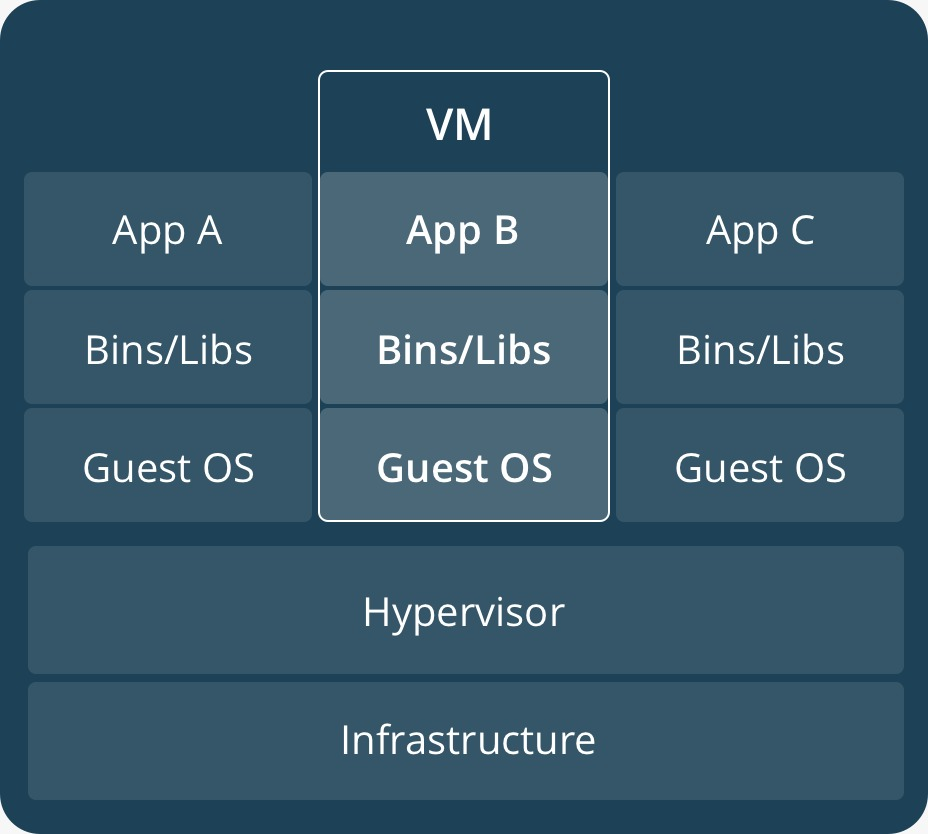
\includegraphics[width=0.4\textwidth]{figures/inkscape/VM.jpeg}}
    \quad
    %\subfloat[]
    {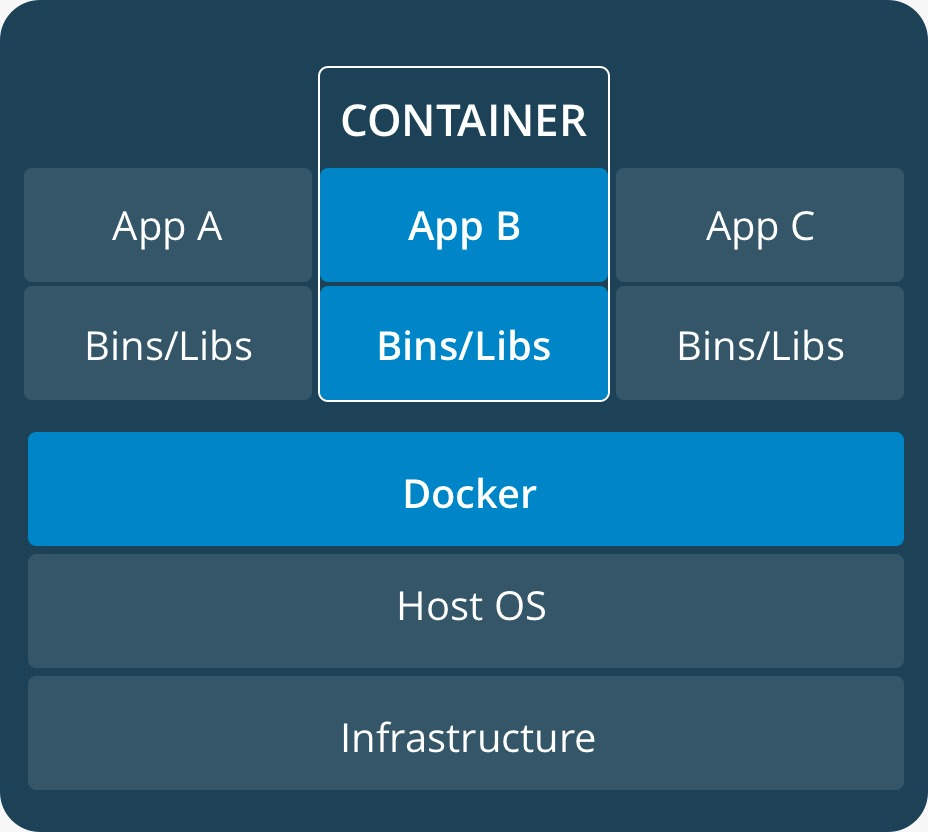
\includegraphics[width=0.4\textwidth ]{figures/inkscape/dockerarchi.jpeg}}
    \caption{Difference between VM and Docker}
    \label{fig:vmvsdocker}

\end{figure}

Docker can also be loosely considered as virtual machine(VM). But unlike a VM, rather than
using a whole operating system, a docker shares the kernel of the system and ships only
the applications that are not in the host machine. Also a docker container is independent
of host machine's applications. This greatly improves performance.

\begin{figure}[!ht]
    \centering
    \def\svgwidth{0.7\textwidth}
    \input{figures/inkscape/dockerfile.pdf_tex}
    \caption{How a docker image is created}
    \label{fig:dockerimage}
\end{figure}
\begin{figure}[!ht]
    \centering
    \def\svgwidth{0.9\textwidth}
    \input{figures/inkscape/docker.pdf_tex}
    \caption{Docker Architecture}
    \label{fig:dockerarchitecure}
\end{figure}

However, docker has its drawbacks. For example, building a docker image sometimes takes
long to compile and consume a lot of resources. So not everyone can build an image as
regularly as they wish.

In this thesis, docker containers are used for data collection from the simulator and later
for evaluation of the model with the simulator.

